\documentclass[a4paper,11pt]{article}
\usepackage[portuguese]{babel}
\usepackage{graphicx}
\usepackage{amsmath}
\usepackage{minted}
\usepackage{mdframed}


\usepackage[twoside,verbose,body={16cm,24cm},
left=25mm,top=20mm]{geometry}


\title{Cálculo de Programas \\ Resolução - Ficha 05}
\author{Eduardo Freitas Fernandes}
\date{2025}

\setminted{
	frame=single,
	tabsize=4,
	breaklines=true
}


\begin{document}
	
	\maketitle
	

	\noindent \underline{\textbf{Exercício 1}}
	\[
	\begin{aligned}
		&id : A \rightarrow B \\
		&\pi_1 : B \times C \rightarrow B \\
		&i_2 : D \rightarrow E + D \\
		&\pi_2 : G \times H \rightarrow H
	\end{aligned}
	\]
	
	\noindent Por $ i_2 \cdot \pi_2 $ inferimos $D = H$:
	\[
	\begin{aligned}
		\frac{
			\frac{
				\begin{array}{c}
					i_2 : D \rightarrow E + D \\
					\pi_2 : G \times H \rightarrow H
				\end{array}
			}
			{
				\begin{array}{c}
					i_2 : D \rightarrow E + D \\
					\pi_2 : G \times D \rightarrow D
				\end{array}
			}
		}
		{
			i_2 \cdot \pi_2 : G \times D \rightarrow E + D
		}
	\end{aligned}
	\]

	\[
	\begin{aligned}
		\frac{
			\begin{array}{c}
				id : A \rightarrow B \\
				\pi_1 : B \times C \rightarrow B
			\end{array}
		}
		{
			id + \pi_1 : A + B \times C \rightarrow A + B
		}
	\end{aligned}
	\]
	
	\noindent Por $ (id + \pi_1) \cdot i_2 \cdot \pi_2 $ inferimos $ A + B \times C = E + D $:
	\[
	\implies
	\begin{cases}
		A = E \\
		B \times C = D
	\end{cases}	
	\]
	
	\[
	\begin{aligned}
		\frac{
			\begin{array}{c}
				id + \pi_1 : A + B \times C \rightarrow A + B \\
				i_2 \cdot \pi_2 : G \times (B \times C) \rightarrow A + B \times C
			\end{array}
		}
		{
			\alpha : G \times (B \times C) \rightarrow A + B
		}
	\end{aligned}
	\]
	
	\noindent \underline{\textbf{Exercício 2}}
	
	\begin{minipage}{0.25\textwidth}
		\[
		\begin{aligned}
			\frac{
				\begin{array}{c}
					join : A + A \rightarrow A \\
					dup : A \rightarrow A \times A
				\end{array}
			}
			{
				\alpha : A + A \rightarrow A \times A
			}
		\end{aligned}
		\]
	\end{minipage}
	\hfill
	\begin{minipage}{0.9\textwidth}
			\begin{figure}[H]
			\centering
			\fbox{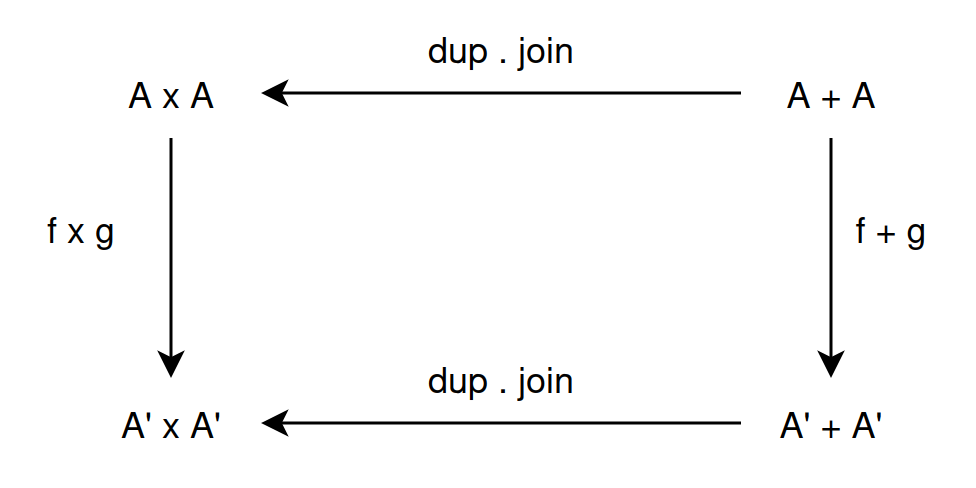
\includegraphics[width=0.5\textwidth]{imgs/cpficha05-2.png}}
		\end{figure}
	\end{minipage}
	
	\noindent Propriedade grátis:
	\[
	(f \times g) \cdot \alpha = \alpha \cdot (f + g)
	\]
	
	\newpage
	
	\noindent \underline{\textbf{Exercício 3}}
	\[
	\begin{aligned}
		& \nabla \cdot (f + f) = f \cdot \nabla \\
		\equiv \  &\{\text{Def-+, Fusão-+}\}\\
		&[\nabla \cdot i_1 \cdot f, \nabla \cdot i_2 \cdot f] = f \cdot \nabla \\
		\equiv \  &\{\text{Universal-+}\}\\
		&\begin{cases}
			\nabla \cdot i_1 \cdot f = f \cdot \nabla \cdot i_1 \\
			\nabla \cdot i_2 \cdot f = f \cdot \nabla \cdot i_2
		\end{cases}\\
		\equiv \  &\{\nabla \cdot i_1 = id, \nabla \cdot i_2 = id \}\\
		&\begin{cases}
			id \cdot f = f \cdot id \\
			id \cdot f = f \cdot id
		\end{cases}\\
		\equiv \  &\{\text{Natural Id}\}\\
		&\begin{cases}
			f = f \\
			f = f
		\end{cases}
	\end{aligned}
	\]
	
	\noindent \underline{\textbf{Exercício 4}}
	\[
	\begin{aligned}
		&f + h: A + B \rightarrow A' + B' \\
		&f + g \times h: A + C \times B \rightarrow A' + C' \times B'
	\end{aligned}
	\]
	
	\begin{figure}[H]
		\centering
		\fbox{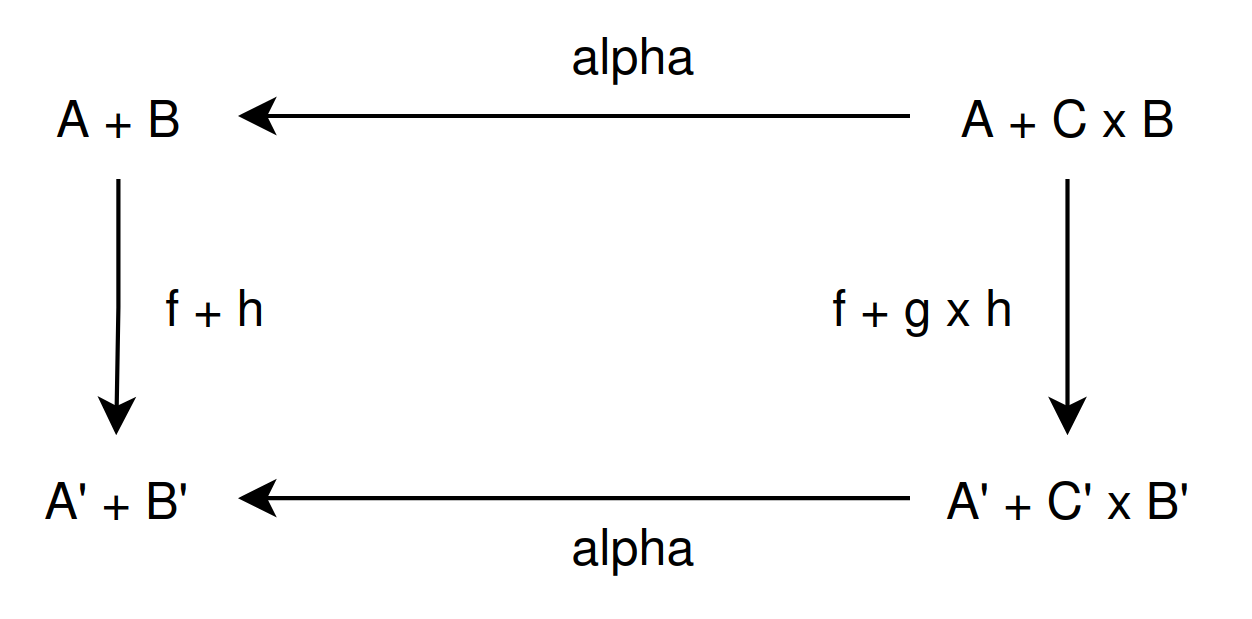
\includegraphics[width=0.5\textwidth]{imgs/cpficha05-4.png}}
	\end{figure}
	
	\[
	\alpha = id + \pi_2
	\]

	\noindent \underline{\textbf{Exercício 5}}
	
	\begin{figure}[H]
		\centering
		\fbox{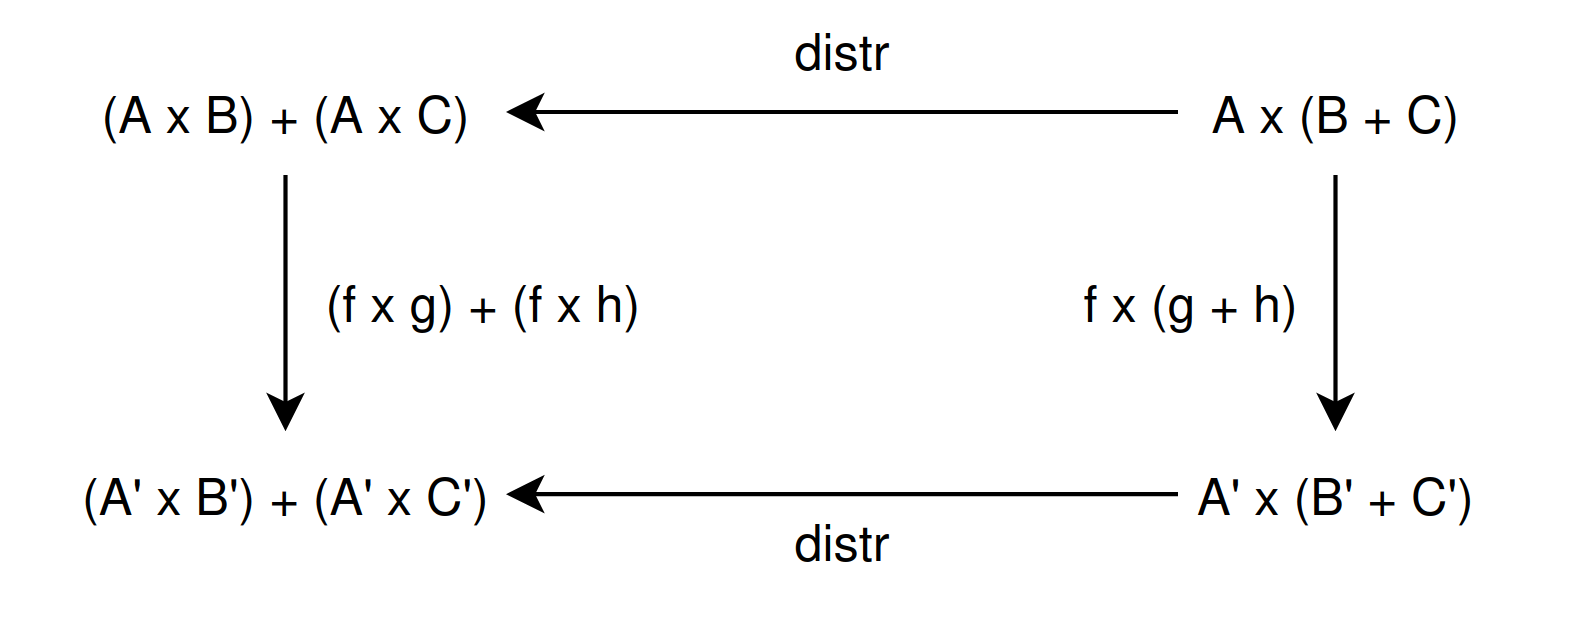
\includegraphics[width=0.5\textwidth]{imgs/cpficha05-distr.png}}
	\end{figure}
	
	\noindent Propriedade grátis:
	\[
	((f \times g) + (f \times h)) \cdot distr = distr \cdot (f \times (g + h))
	\]
	
	\[
	\begin{aligned}
		& h \cdot distr \cdot (g \times (id + f)) = k \\
		\equiv \  &\{\text{propriedade grátis}\}\\
		& h \cdot ((g \times id) + (g \times f)) \cdot distr = k \\
		\equiv \  &\{\text{(F6)}\}\\
		& h \cdot ((g \times id) + (g \times f)) = k \cdot distr^{\circ} \\
		\equiv \  &\{\text{$distr^{\circ} = undistr$}\}\\
		& h \cdot ((g \times id) + (g \times f)) = k \cdot undistr \\
	\end{aligned}
	\]
	
	\noindent \underline{\textbf{Exercício 6}}
	\[
	\begin{aligned}
		&(p \cdot h) \rightarrow (f \cdot h), (g \cdot h) \\
		\equiv \  &\{\text{Def condicional de McCarthy}\}\\
		& [f \cdot h, g \cdot h] \cdot (p \cdot h)? \\
		\equiv \  &\{\text{Absorção-+}\}\\
		& [f, g] \cdot (h + h) \cdot (p \cdot h)? \\
		\equiv \  &\{\text{Natural-guarda}\}\\
		& [f, g] \cdot p? \cdot h \\
		\equiv \  &\{\text{Def condicional de McCarthy}\}\\
		& (p \rightarrow f, g) \cdot h \\
	\end{aligned}
	\]
	
	\noindent \underline{\textbf{Exercício 7}}
	\[
	\begin{aligned}
		& choose \cdot parallel p f g = p \rightarrow f, g \\
		\equiv \  &\{\text{def. parallel, def. choose}\}\\
		& (\pi_2 \rightarrow \pi_1 \cdot \pi_1, \pi_2 \cdot \pi_1) \cdot \langle \langle f, g \rangle, p \rangle = p \rightarrow f, g \\
		\equiv \  &\{\text{Def condicional de McCarthy}\}\\
		& [\pi_1 \cdot \pi_1, \pi_2 \cdot \pi_1] \cdot \pi_2 ? \cdot \langle \langle f, g \rangle, p \rangle = p \rightarrow f, g \\
		\equiv \  &\{\text{Natural-guarda }\}\\
		& [\pi_1 \cdot \pi_1, \pi_2 \cdot \pi_1] \cdot ( \langle \langle f, g \rangle, p \rangle + \langle \langle f, g \rangle, p \rangle ) \cdot (\pi_2 \cdot \langle \langle f, g \rangle, p \rangle)? = p \rightarrow f, g \\
		\equiv \  &\{\text{Cancelamento-$\times$, Absorção-+}\}\\
		& [\pi_1 \cdot \pi_1 \cdot \langle \langle f, g \rangle, p \rangle , \pi_2 \cdot \pi_1 \cdot \langle \langle f, g \rangle, p \rangle] \cdot p? = p \rightarrow f, g \\
		\equiv \  &\{\text{Cancelamento-$\times$}\}\\
		& [f, g] \cdot p? = p \rightarrow f, g \\
		\equiv \  &\{\text{Def condicional de McCarthy}\}\\
		& p \rightarrow f, g = p \rightarrow f, g \\
	\end{aligned}
	\]
	
	\newpage
	
	\noindent \underline{\textbf{Exercício 8}}\\
	
	\noindent \textbf{Primeira} propriedade:
	\[
	\begin{aligned}
		& \langle (p \rightarrow f, h), (p \rightarrow g, i) \rangle \\
		\equiv \  &\{\text{Def condicional de McCarthy (2*)}\}\\
		& \langle [f, h] \cdot p?, [g, i] \cdot p? \rangle \\
		\equiv \  &\{\text{Fusão-$\times$}\}\\
		& \langle [f, h] , [g, i] \rangle \cdot p? \\
		\equiv \  &\{\text{Lei da troca}\}\\
		& [\langle f, g \rangle, \langle h, i \rangle] \cdot p? \\
		\equiv \  &\{\text{Def condicional de McCarthy}\}\\
		& p \rightarrow \langle f, g \rangle, \langle h, i \rangle \\
	\end{aligned}
	\]
	
	\noindent \textbf{Segunda} propriedade:
	\[
	\begin{aligned}
		&p \rightarrow \langle f, g \rangle, \langle f, h \rangle \\
		\equiv \  &\{\text{(F11)}\}\\
		& \langle (p \rightarrow f, f), (p \rightarrow g, h) \rangle \\
		\equiv \  &\{\text{(F9)}\}\\
		& \langle f, (p \rightarrow g, h) \rangle \\
	\end{aligned}
	\]
	
	\noindent \textbf{Terceira} propriedade:
	\[
	\begin{aligned}
		&p \rightarrow (p \rightarrow a, b) , (p \rightarrow c, d) \\
		\equiv \  &\{\text{Def condicional de McCarthy (3*)}\}\\
		& [[a, b] \cdot p?, [c, d] \cdot p?] \cdot p? \\
		\equiv \  &\{\text{Absorção-+}\}\\
		& [[a, b], [c, d]] \cdot (p? + p?) \cdot p? \\
		\equiv \  &\{\text{(F10)}\}\\
		& [[a, b], [c, d]] \cdot (i1 + i2) \cdot p? \\
		\equiv \  &\{\text{Absorção-+, Cancelamento-+}\}\\
		& [a, d] \cdot p? \\
		\equiv \  &\{\text{Def condicional de McCarthy}\}\\
		& p \rightarrow a, d \\
	\end{aligned}
	\]
	
	\noindent \underline{\textbf{Exercício 9}}
	
\begin{minted}{haskell}
f :: (Eq a) => [a] -> Either a (a, [a])
f = undefined
\end{minted}
	
	
\end{document}
